\documentclass[a4paper,USenglish,cleveref,autoref,thm-restate]{lipics-v2021}
\nolinenumbers

\title{Saturation Problems for Families of Automata}

\author{León Bohn}{RWTH Aachen University, Germany}{bohn@lics.rwth-aachen.de}{https://orcid.org/0000-0003-0881-3199}{Supported by DFG grant LO 1174/7-1}
\author{Yong Li}{Key Laboratory of System Software (Chinese Academy of Sciences) and State Key Laboratory of Computer Science, Institute of Software, Chinese Academy of Sciences, PRC}{liyong@ios.ac.cn}{https://orcid.org/0000-0002-7301-9234}{Supported by National Natural Science Foundation of China (Grant No. 62102407)}
\author{Christof Löding}{RWTH Aachen University, Germany}{loeding@automata.rwth-aachen.de}{https://orcid.org/0000-0002-1529-2806}{}
\author{Sven Schewe}{University of Liverpool, UK}{sven.schewe@liverpool.ac.uk}{https://orcid.org/0000-0002-9093-9518}{Supported by the EPSRC through projects EP/X03688X/1 and EP/X042596/1}

\authorrunning{L. Bohn, Y. Li, C. Löding, S. Schewe}
\Copyright{León Bohn, Yong Li, Christof Löding, and Sven Schewe}

\ccsdesc[100]{Theory of computation~Automata over infinite objects}
\keywords{Families of Automata, automata learning, FDFAs}
\category{Track B: Automata, Logic, Semantics, and Theory of Programming}
\EventEditors{Keren Censor-Hillel, Fabrizio Grandoni, Joel Ouaknine, and Gabriele Puppis}
\EventNoEds{4}
\EventLongTitle{52nd International Colloquium on Automata, Languages, and Programming (ICALP 2025)}
\EventShortTitle{ICALP 2025}
\EventAcronym{ICALP}
\EventYear{2025}
\EventDate{July 8--11, 2025}
\EventLocation{Aarhus, Denmark}
\EventLogo{}
\SeriesVolume{334}
\ArticleNo{151}


\bibliographystyle{plainurl}

\usepackage[table,dvipsnames]{xcolor}
\usepackage{xspace}

\usepackage{amssymb,amsmath,amsthm}
\usepackage{mathtools,thmtools} 
\usepackage{tikz}
\usetikzlibrary{shapes.geometric, decorations, calc,arrows,decorations.pathreplacing}
\usetikzlibrary {arrows.meta}
\usetikzlibrary{decorations.pathmorphing}
\usetikzlibrary{automata,positioning}

\tikzset{
    box/.style={
        draw,
        rectangle,
        minimum width=2cm,
        minimum height=1cm,
        text centered,
        node distance=3cm,
    },
    softbox/.style={
        draw,
        rectangle,
        rounded corners=8pt,
        minimum width=2cm,
        minimum height=1cm,
        text centered,
        node distance=3cm,
        thick
    },
    rounded/.style={
        draw,
        ellipse,
        minimum width=2cm,
        minimum height=1cm,
        text centered,
        node distance=3cm,
    },
    squiggly/.style={
        decorate,
        decoration={
            snake,
            amplitude=.4mm,
            segment length=2mm,
            post length=1mm,
            pre length=1mm
        },
        thick
    }
}

\tikzset{automaton/.append style={
			shorten >=1pt,
			auto,
			on grid,
			node distance=10mm,
			initial text=,
			every edge/.append style={
					every node/.append style={
							font=\scriptsize
						}
				},
			every state/.append style={
					inner sep=1pt,
					minimum size=3mm,
                    font=\small,
                    draw=none,
				},
			squig/.append style={decorate,decoration={snake, amplitude=0.2mm, segment length=1.5mm}}
		},
        lblsmall/.append style={
            every node/.append style={
                font=\small
            },
			every edge/.append style={
					every node/.append style={
							font=\small
						}
				},
        },
        lbltiny/.append style={
            every node/.append style={
                font=\scriptsize
            },
			every edge/.append style={
					every node/.append style={
							font=\scriptsize
						}
				},
        }
}

 
\usepackage{mathcommand}
\usepackage[notion, quotation,hyperref,electronic]{knowledge}

\declaretheorem[name=Lemma,sibling=lemma]{rstlemma}
\declaretheorem[name=Corollary,sibling=corollary]{rstcorollary}
\declaretheorem[name=Theorem,sibling=theorem]{rsttheorem}

\definecolor{blueish}{RGB}{0,84,159}
\definecolor{petrolish}{RGB}{0,97,101}
\definecolor{violett}{RGB}{97,33,88}

\definecolor{primary}{rgb}{0.0,0.25,0.42}
\newcommand{\primary}[1]{{\color{primary}#1}}
\definecolor{secondary}{rgb}{0.44, 0.11, 0.11}
\newcommand{\secondary}[1]{{\color{secondary}#1}}
\definecolor{tertiary}{rgb}{0.32,0.18,0.5}
\newcommand{\tertiary}[1]{{\color{tertiary}#1}}
\definecolor{quartary}{rgb}{0.45,0.42,0.75}
\newcommand{\quartary}[1]{{\color{quartary}#1}}

\newcommand{\red}[1]{{\color{red} #1}}

\newcommand{\mc}[1]{\ensuremath{\mathcal{#1}}}
\newcommand{\mf}[1]{\ensuremath{\mathfrak{#1}}}
\newcommand{\mb}[1]{\ensuremath{\mathbb{#1}}}
\renewcommand{\sf}[1]{\ensuremath{\mathsf{#1}}}

\newcommand{\reprs}[1][\Sigma]{\ensuremath{{#1}^* \times {#1}^+}}
\newcommand{\loops}[2]{\ensuremath{\LangDFA{\DFA{#1, #1(#2), \{#1(#2)\}}}}}

\newcommand{\A}{\mc{A}}
\newcommand{\T}{\mc{T}}
\newcommand{\F}{\mc{F}}
\newcommand{\M}{\mc{M}}
\newcommand{\N}{\mc{N}}
\newcommand{\D}{\mc{D}}
\newcommand{\C}{\mc{C}}
\renewcommand{\L}{\mc{L}}
\newcommand{\B}{\mc{B}}
\newcommand{\W}{\mc{W}}
\renewcommand{\P}{\mc{P}}

\newcommand{\Dmin}{\mc{D}^{\mathsf{min}}}
\newcommand{\Fnc}{\mc{F}^\mathsf{nc}}

\newcommand{\eps}{\ensuremath{\varepsilon}}

\newcommand{\op}[1]{\ensuremath{\operatorname{\mathsf{#1}}}}

\newcommand{\true}{\mathsf{true}}
\newcommand{\false}{\mathsf{false}}

\newcommand{\bigO}{\mathcal{O}}

\newcommand{\SSP}{\Sigma^{*} \times \Sigma^+}

\newcommand{\id}{\mathop{\operatorname{\mathsf{id}}}}

\newcommand{\NL}{\textsf{NL}\xspace}
\newcommand{\NLcomplete}{\textsf{NL}-complete\xspace}
\newcommand{\PSPACE}{\textsf{PSPACE}\xspace}
\newcommand{\PTIME}{\textsf{PTIME}\xspace}
\newcommand{\PSPACEcomplete}{\textsf{PSPACE}-complete\xspace}

\newcommand{\PHP}{\ensuremath{\textsf{PHP}_{\eps}}\xspace}

\newcommand{\powroot}[1]{\ensuremath{\left(\sqrt{#1}\right)^+}}


\newcommand{\moracle}{\textit{mem}}
\newcommand{\eoracle}{\textit{eq}}

\newcommand{\Sat}{\mathsf{Sat}} 

\IfKnowledgePaperModeTF{
}{
\knowledgestyle{intro notion}{color={secondary}, emphasize}
  \knowledgestyle{notion}{color={primary}}
  \hypersetup{
    colorlinks=true,
    breaklinks=true,
    linkcolor={tertiary}, citecolor={quartary}, }
}
\knowledgeconfigureenvironment {proof}{}

\knowledge{notion}
| ultimately periodic
| ultimately periodic word
\knowledgenewrobustcmd{\UP}[1]{\mathop{\cmdkl{\mathsf{UP}}}(#1)}

\knowledge{notion}
| loop
| loops

\knowledge{notion}
| transition system
| TS
\knowledgenewrobustcmd{\states}[1]{\mathop{\cmdkl{Q}}(#1)}
\knowledge{notion}
| size@TS

\knowledge{notion}
| strongly connected component
| strongly connected components

\knowledge{notion}
| deterministic finite automaton
| DFA
| DFAs
\knowledgenewrobustcmd{\DFA}[1]{\mathop{\cmdkl{\mathsf{DFA}}}(#1)}
\knowledgenewrobustcmd{\LangDFA}[1]{\mathop{\cmdkl{L_*}}(#1)}
\knowledge{notion}
| nondeterministic finite automaton
| NFA

\knowledge{notion}
| Moore machine

\knowledge{notion}
| regular
| regular $\omega$-language
| regular $\omega$-languages

\knowledge{notion}
| UP-regular

\knowledge{notion}
| UP-equivalent

\knowledge{notion}
| deterministic Büchi automaton
| DBA

\knowledgenewrobustcmd{\LangDBA}[1]{\mathop{L_\omega}(#1)}

\knowledge{notion}
| weak

\knowledge{notion}
| nondeterministic Büchi automaton
| NBA

\let\root\undefined
\knowledgenewrobustcmd{\wordroot}[1]{\cmdkl{\sqrt{#1}}}
\knowledge{synonym}
| root

\knowledgenewrobustcmd{\Pow}[1]{\cmdkl{\operatorname{\omega-\mathsf{Pow}}}(#1)}

\knowledge{notion}
| prefix-independent
| $\sim_L$ is trivial

\knowledge{notion}
| family of deterministic finite automata
| FDFA
| FDFAs

\knowledge{notion}
| leading transition system
| leading TS

\knowledge{notion}
| progress DFA
| progress DFAs

\knowledge{notion}
| syntactic FDFA

\knowledge{notion}
| family of right congruences
| FORC

\knowledge{notion}
| refines

\knowledge{notion}
| language recognizing FORC
| LFORC

\knowledge{notion}
| normalized (with regard to $\F$)
| loops on $u$
| loops on
| loop on
| loops on some class
| normalized

\knowledgenewrobustcmd{\ReprFDFA}[1]{\mathop{\cmdkl{{\mathsf{L}}_{\mathsf{rep}}}}(#1)}
\knowledgenewrobustcmd{\NormFDFA}[1]{\mathop{\cmdkl{{\mathsf{L}}_{\mathsf{norm}}}}(#1)}
\knowledge{notion}
| language@FDFA
| accepted@FDFA
| accepts@FDFA
\knowledgenewrobustcmd{\LangFDFA}[1]{\mathop{\cmdkl{L_\omega}}(#1)}

\knowledgenewrobustcmd{\ReprFDWA}[1]{\mathop{\cmdkl{{\mathsf{L}}_{\mathsf{rep}}}}(#1)}
\knowledgenewrobustcmd{\NormFDWA}[1]{\mathop{\cmdkl{{\mathsf{L}}_{\mathsf{norm}}}}(#1)}
\knowledge{notion}
| language@FDWA
| accepts@FDWA
\knowledgenewrobustcmd{\LangFDWA}[1]{\mathop{\cmdkl{L_\omega}}(#1)}

\knowledge{notion}
| family
| families

\knowledge{notion}
| prefix-independent@family
\knowledge{notion}
| size@family
\knowledge{notion}
| language@family

\knowledgenewmathcommandPIE{\redequiv}{\mathrel{\cmdkl{\equiv#2#3}}}

\knowledge{notion}
| saturated for $\X$

\knowledge{notion}
| saturated
| saturation
| Saturation
| saturated FDFA
| saturated FDFAs
| saturated FDWA
| Saturated FDWAs
| saturated FDWAs

\knowledge{notion}
| almost saturated
| almost saturation
| almost saturated FDFA
| almost saturated FDFAs

\knowledge{notion}
| full saturation
| fully saturated
| fully saturated FDFA
| fully saturated FDFAs

\knowledge{notion}
| reference set

\knowledge{notion}
| loopshift-stable
| loopshift-stability

\knowledge{notion}
| loopshift-stable@for
| loopshift-stability@for
| loopshift-stable for $\X$
| loopshift-stable for

\knowledge{notion}
| power-stable
| power-stability

\knowledge{notion}
| power-stable@for
| power-stability@for
| power-stable for $\X$
| power-stable for

\knowledge{notion}
| upward power-stable

\knowledge{notion}
| family of deterministic weak automata
| FDWA
| FDWAs

\knowledge{notion}
| progress automaton

\knowledge{notion}
| Transition profiles
| transition profile

\knowledge{notion}
| active learner

\knowledge{notion}
| passive learner

\knowledge{notion}
| membership oracle

\knowledge{notion}
| equivalence oracle

\knowledge{notion}
| target language







 

\newcommand{\ifappendix}[1]{\ifappendixelse{#1}{}}
\newcommand{\ifnotappendix}[1]{\ifappendixelse{}{#1}}
\newcommand{\ifappendixelse}[2]{\ifthenelse{\isundefined{\shouldhaveappendix}}{#2}{#1}}
\newcommand*{\shouldhaveappendix}{}

\newcommand{\iftodoselse}[2]{\ifthenelse{\isundefined{\showtodos}}{#2}{#1}}

\iftodoselse{\usepackage{todonotes}
\newcommand{\sven}[1]{\todo[inline,color=teal!10,caption={Sven}]{\textbf{Sven:}
#1}}
\newcommand{\ly}[1]{\todo[inline,color=orange!10,caption={LY}]{\textbf{LY:} #1}}
\newcommand{\leon}[1]{\todo[color=green!10,caption={Leon}]{\textbf{Leon:} #1}}
\newcommand{\leonin}[1]{\todo[inline,color=green!10,caption={Leon}]{\textbf{Leon:} #1}}
\newcommand{\chrin}[1]{\todo[inline,color=Orchid!30,caption={Christof}]{\textbf{Christof:} #1}}
\newcommand{\chr}[1]{\todo[color=Orchid!30,caption={Christof}]{\textbf{Christof:} #1}}
}{\newcommand{\sven}[1]{}
\newcommand{\ly}[1]{}
\newcommand{\leon}[1]{}
\newcommand{\leonin}[1]{}
\newcommand{\chr}[1]{}
\newcommand{\chrin}[1]{}
}


\begin{document}

\maketitle


\begin{abstract}
Families of deterministic finite automata (FDFA) represent regular $\omega$-languages through their ultimately periodic words (UP-words).
An FDFA accepts pairs of words, where the first component corresponds to a prefix of the UP-word, and the second component represents a period of that UP-word.
An FDFA is termed saturated if, for each UP-word, either all or none of the pairs representing that UP-word are accepted.
We demonstrate that determining whether a given FDFA is saturated can be accomplished in polynomial time, thus improving the known \PSPACE upper bound by an exponential.
We illustrate the application of this result by presenting the first polynomial learning algorithms for representations of the class of all regular $\omega$-languages.
Furthermore, we establish that deciding a weaker property, referred to as almost saturation, is \PSPACE-complete.
Since FDFAs do not necessarily define regular $\omega$-languages when they are not saturated, we also address the regularity problem and show that it is \PSPACE-complete.
Finally, we explore a variant of FDFAs called families of deterministic weak automata (FDWA), where the semantics for the periodic part of the UP-word considers $\omega$-words instead of finite words. 
We demonstrate that saturation for FDWAs is also decidable in polynomial time, that FDWAs always define regular $\omega$-languages, and we compare the succinctness of these different models.
\end{abstract} \section{Introduction}
\label{section:introduction}
Regular $\omega$-languages (languages of infinite words) are a useful tool for developing decision procedures in logic that have applications in model checking and synthesis~\cite{BaierK2008,Thomas09}. There are many different formalisms for representing regular $\omega$-languages, like regular expressions, automata, semigroups, and logic~\cite{Thomas90,PerrinP04}. In this paper, we study \emph{families of automata} that represent regular $\omega$-languages in terms of the ultimately periodic words that they contain.  This is based on the fact that a regular $\omega$-language is uniquely determined by the ultimately periodic words that it contains, which follows from results by Büchi \cite{Buchi62} on the closure of regular $\omega$-languages under Boolean operations (see also \cite[Fact~1]{CalbrixNP93})).  Ultimately periodic words are of the form $uv^\omega$ for finite words $u,v$ (where $v$ is non-empty). For a regular $\omega$-language $L$, \cite{CalbrixNP93} considers the language $L_\$$ of all finite words of the form $u\$ v$ with $uv^\omega \in L$. They show that $L_\$$ is regular, and from a DFA for $L_\$$ one can construct in polynomial time a nondeterministic B\"uchi automaton for $L$.
A similar approach was used independently by Klarlund in \cite{Klarlund94} who introduces the concept of \emph{families of deterministic finite automata} (FDFA) for representing $\omega$-languages, based on the notion of family of right congruences (FORC) introduced by Maler and Staiger \cite{MalerS97}. Instead of using a single DFA, an FDFA consists of one so-called leading transition system, and so-called progress DFAs, one for each state of the leading transition system.
A pair $(u,v)$ of finite words (with $v$ non-empty) is accepted if $v$ is accepted by the progress DFA of the state reached by $u$ in the leading transition system. As opposed to the $L_\$$ representation from \cite{CalbrixNP93}, the FDFA model of \cite{Klarlund94,MalerS97} only considers pairs $(u,v)$ such that $v$ loops on the state of the leading transition system that is reached by $u$, referred to as \emph{normalized pairs}. So an FDFA for $L$ is an FDFA that accepts all normalized pairs $(u,v)$ with $uv^\omega \in L$. 

Because there exist many learning algorithms for DFAs, these kinds of representations based on DFAs have received attention in the area of learning regular $\omega$-languages
\cite{FarzanCCTW08,AngluinF16,LiCZL21,BohnL22,BohnL24,LiST24}. 
One problem is that methods for DFA learning might come up with automata that treat different pairs that define the same ultimately periodic word differently. So it might happen that a pair $(u_1,v_1)$ is accepted while $(u_2,v_2)$ is rejected, although $u_1v_1^\omega = u_2v_2^\omega$. In this case it is not clear anymore which $\omega$-language is accepted. One can use the existential (nondeterministic) semantics and say that $uv^\omega$ is accepted if some pair representing $uv^\omega$ is accepted. But this does not necessarily define a regular $\omega$-language (see \cite[Example 2]{LiCZL21}).
An FDFA is called \emph{saturated} if it treats all normalized pairs representing the same ultimately periodic word in the same way (accepts all or rejects all). Additionally, we call an FDFA \emph{fully saturated} if it treats all pairs representing the same ultimately periodic words in the same way (not only the normalized ones). The $u\$v$ representation corresponds to fully saturated FDFAs because a DFA for the language $L_\$$ can easily be turned into a fully saturated FDFA for $L$ by taking the part before $\$$ as leading transition system, and the part after the $\$$ for defining the progress DFAs.

It has been shown in \cite{AngluinBF18} that saturated FDFAs possess many good properties as formalism for defining $\omega$-languages.\footnote{The semantics of FDFAs in \cite{AngluinBF18} and \cite{Klarlund94} are defined differently, however, saturated FDFAs define the same $\omega$-languages in both models. We follow the definitions from \cite{AngluinBF18}.} However, up to now the best known upper bound on the complexity for deciding if a given FDFA is (fully) saturated is \PSPACE \cite{AngluinBF18}. In this paper, we settle several questions concerning the complexity of saturation problems. 
As our first contribution we provide polynomial time algorithms for deciding saturation and full saturation of FDFAs, solving a question that was first posed more than three decades ago in \cite{CalbrixNP93} (see related work for existing work on the saturation problem). 
We also consider the property of almost saturation, which is weaker than saturation and thus allows for smaller FDFAs (\Cref{lemma:lowerbound:combinedToSatFDFA}), while ensuring that almost saturated FDFAs define regular $\omega$-languages \cite{LiST23}. We show that this comes at a price, because deciding almost saturation is \PSPACE-complete. Furthermore, we show that it is \PSPACE-complete to decide whether a given FDFA defines a regular $\omega$-language, solving a question that was raised in \cite{CalbrixN95}.

An overview of the models that appear in our paper and of our results is given in Figure~\ref{fig:overview}. The different classes of FDFAs are shown on the left-hand side. The entries \PTIME/\PSPACE-c.\ indicate the complexity of deciding whether a given FDFA belongs to the respective class. As an application of the polynomial saturation algorithms, we provide the \emph{first} polynomial learning algorithms for classes representing all regular $\omega$-languages: a polynomial time active learner for fully saturated FDFAs, and a passive learner for syntactic FDFAs that is polynomial in time and data (see related work for existing work on learning $\omega$-languages). The syntactic FDFA for $L$ is the saturated FDFA with the least possible leading transition system (called $\mathfrak{L}^L$ in \cite{Klarlund94}). 
The size of the models that our algorithms can learn is, in general, incomparable to the size of deterministic parity automata (DPAs) (\cite[Theorem~5.12]{AngluinBF18} shows an exponential lower bound from saturated FDFAs to DPAs and the language family used for that is accepted also by small fully saturated FDFAs; an exponential lower bound from DPAs to syntactic FDFAs follows from the language family $L_n$ used in  \Cref{lemma:expgapsatFDFAsynFDFAfullysatFDFA}, which is easily seen to be accepted by small DPAs).
\begin{figure}
    \begin{center}
    \begin{tikzpicture}[baseline={(NBA)},box/.style={draw,rectangle,minimum width=0.3\textwidth,text centered,node distance=3cm,inner sep=3pt,},softbox/.style={draw,rectangle,dash dot,rounded corners=10pt,minimum width=0.4\textwidth,minimum height=1cm,text centered,node distance=3cm,minimum width=0.3\textwidth,},rounded/.style={draw,ellipse,
text centered,node distance=3cm,}]
        \node[box] (fullysatFDFA) {\begin{tabular}{c}"fully saturated FDFA"\end{tabular}};
        \node[box, below=0.05\textheight of fullysatFDFA] (synFDFA) {\begin{tabular}{c}"syntactic FDFA"\end{tabular}};
        \node[box, below=0.05\textheight of synFDFA] (satFDFA) {\begin{tabular}{c}"saturated FDFA"\end{tabular}};
        \node[box, below=0.05\textheight of satFDFA] (almostsatFDFA) {\begin{tabular}{c}"almost saturated FDFA"\end{tabular}};
        \node[box, minimum width=0.15\textwidth, below=0.05\textheight of almostsatFDFA] (FDFA) {"FDFA"};

        \node[softbox,right=0.25\textwidth of fullysatFDFA] (ptimeAL) {\begin{tabular}{c}polynomial-time\\active learner\end{tabular}};
        \node[softbox] (passiveLearner) at (synFDFA -| ptimeAL) {\begin{tabular}{c}passive learner\\polynomial time\\and polynomial data\end{tabular}};
        
        \node[box] (satFDWA) at ($(satFDFA)!0.5!(almostsatFDFA) + (0.5\textwidth,0)$) {\begin{tabular}{c}"saturated FDWA"\end{tabular}};
        \node[box, minimum width=0.15\textwidth] (FDWA) at ($(FDFA -| satFDWA) + (0,.04\textheight)$) {"FDWA"};

        \node[rounded] (NBA) at ($(FDFA)!0.5!(FDWA) + (0,-0.025\textwidth)$) {"NBA"};       

        \tikzset{lblsmall}

\draw[-, double](fullysatFDFA) edge node[anchor=south]{Thm~\ref{theorem:activelearner}} (ptimeAL);
        \draw[-, double](synFDFA) edge node[anchor=south]{Thm~\ref{theorem:passivelearner}} (passiveLearner);

\draw[densely dotted, thick]
        (FDWA.west) edge[->, bend right=10] node[anchor=north west] {\small Lem~\ref{lemma:FDWAregular}} (NBA)
        (almostsatFDFA.east) edge[->, bend left=20] node[anchor=west] {\small \cite{LiST23}}  (NBA)
        ;

\draw[->]
        (fullysatFDFA) edge[transform canvas={xshift=-4mm}] (synFDFA)
        (synFDFA) edge[transform canvas={xshift=-4mm}] (satFDFA)
        (satFDFA) edge[transform canvas={xshift=-4mm}] (almostsatFDFA)
        (almostsatFDFA) edge[transform canvas={xshift=-4mm}] (FDFA)
        (satFDWA) edge[transform canvas={xshift=-4mm}]  (FDWA);

\draw[->, dashed, lblsmall]
        (synFDFA) edge[bend left=10,transform canvas={xshift=-4mm}] node[anchor=east] {\begin{tabular}{c}Lem~\ref{lemma:expgapsatFDFAsynFDFAfullysatFDFA}\\\cite[Thm~2]{AngluinF16} \end{tabular}} (fullysatFDFA)
        (satFDFA) edge[bend left=10,transform canvas={xshift=-4mm}] node[anchor=east] {\begin{tabular}{c}Lem~\ref{lemma:expgapsatFDFAsynFDFAfullysatFDFA}\\\cite[Sec~5]{Klarlund94}\end{tabular}} (synFDFA)
        (almostsatFDFA) edge[bend left=10,transform canvas={xshift=-4mm}] node[anchor=east] {Lem~\ref{lemma:lowerbound:combinedToSatFDFA}} (satFDFA)
        (satFDWA) edge[bend left=5] node[anchor=north east] {Lem~\ref{lemma:lowerbound:combinedToSatFDFA}} (satFDFA.east)
        (almostsatFDFA) edge[bend right=4] node[anchor=south] {Lem~\ref{lemma:incomparableSatFDWAalsatFDFA}} (satFDWA)
        (satFDWA) edge[bend right=4] (almostsatFDFA)
        (FDWA) edge[bend left=10,transform canvas={xshift=-4mm}] node [anchor=east] {Lem~\ref{lemma:incomparableSatFDWAalsatFDFA}} (satFDWA);

\draw[lblsmall]
        (satFDFA.east) edge[->, bend left=10] node[anchor=south] {\small \cite[Sec~4]{BohnL24}} (satFDWA.north);

\draw[->]
        (fullysatFDFA) to [out=175, in=185, looseness=4] node[anchor=west] {c.} (fullysatFDFA);
        \draw[->]
        (synFDFA) to [out=175, in=185, looseness=4] node[anchor=west] {c.}  (synFDFA);
        \draw[->]        
        (satFDFA) to [out=175, in=185, looseness=4] node[anchor=west] {c.}  (satFDFA);
\draw[->]
        (satFDWA) to [out=355, in=5, looseness=4] node[anchor=east] {c.} (satFDWA);
        \draw[->, dashed]
        (almostsatFDFA) to [out=175, in=185, looseness=4] node[anchor=west] {c.} node[anchor=north,overlay,yshift=-3mm] {\small Lem~\ref{lemma:incomparableSatFDWAalsatFDFA}} (almostsatFDFA);

\node[inner sep=1pt, draw=black, dotted, anchor=north east] (DECfullysatFDFA) at (fullysatFDFA.south east) {\scriptsize \PTIME (Thm~\ref{theorem:ptimesaturationFDFA})};
        \node[inner sep=1pt, draw=black, dotted, anchor=north east] (DECsynFDFA) at (synFDFA.south east) {\scriptsize \PTIME (Thm~\ref{theorem:ptimesaturationFDFA})};
        \node[inner sep=1pt, draw=black, dotted, anchor=north east] (DECsatFDFA) at (satFDFA.south east) {\scriptsize \PTIME (Thm~\ref{theorem:ptimesaturationFDFA})};
        \node[inner sep=1pt, draw=black, dotted, anchor=north east] (DECalmostsatFDFA) at (almostsatFDFA.south east) {\scriptsize \PSPACE-c. (Thm~\ref{theorem:powerclosednessPSPACEcomplete})};
\node[inner sep=1pt, draw=black, dotted, anchor=north east] (DECsatFDWA) at (satFDWA.south east) {\scriptsize \PTIME (Thm~\ref{theorem:ptimesaturationFDWA})};
    \end{tikzpicture}
    \caption{Overview of the properties and models considered in this paper. 
    Solid arrows indicate translations that are possible without blowup, while dashed ones are used for translations with an exponential lower bound.
    Dotted arrows are constructions yielding automata, and ones labeled with ``c.'' are complementation constructions.
    Solid lines are used to indicate a connection to learning.
    We provide more details on this diagram in the introduction.}
\label{fig:overview}
    \end{center}
\end{figure} 
For completing the picture of the FDFA landscape, we also give examples showing that complementing almost saturated FDFAs can cause an exponential blow-up (while it is trivial for saturated or fully saturated FDFAs), and for exponential size gaps between the different models. Exponential lower bounds are indicated by the dashed arrows in Figure~\ref{fig:overview}, where the loops labeled ``c.''~represent the complement. The solid arrows mean that there is a transformation that does not cause any blow-up. 

Finally, we also consider the model of families of deterministic weak automata (FDWA), which is shown with two entries on the right-hand side of Figure~\ref{fig:overview}. This is an automaton model for families of weak priority mappings (FWPM), which have been introduced in \cite{BohnL24}. Syntactically, an FDWA is an FDFA in which the progress DFAs have the property that each strongly connected component (SCC) of states is either completely accepting or completely rejecting. This corresponds to the restriction made for deterministic weak (B\"uchi) automata (DWA); See, e.g., \cite{Loding01}. And indeed, the progress automata are not interpreted as DFAs accepting finite words, but as deterministic weak automata accepting periodic words: a pair $(u,v)$ is accepted if $v^\omega$ is accepted by the progress DWA of the state reached by $u$ in the leading transition system, which means that $v^\omega$ ends up cycling in an accepting SCC. 
As for FDFAs, the property of saturation for FDWAs requires that either all normalized representations of an ultimately periodic word are accepted or none. (In order to not consider too many models, we restricted ourselves to existing ones and did not additionally introduce fully saturated and syntactic FDWAs.)
We show that saturation can also be decided in polynomial time for FDWAs, which is easier to see than for FDFAs.

Concerning succinctness of FDWAs compared to FDFAs, it follows from results in \cite{BohnL24} that saturated FDFAs can be transformed into saturated FDWAs by only adapting the acceptance mechanism and keeping the transition structure. We show that a translation in the other direction can cause an exponential blow-up, even when going to the more relaxed model of almost saturated FDFAs. Vice versa, we show that translating almost saturated FDFAs to saturated FDWAs also might cause an exponential blow-up.



In summary, our contributions are polynomial saturation algorithms for FDFAs and FDWAs, \PSPACE-completeness results for deciding almost saturation and regularity of FDFAs, and some exponential lower bounds for
transformations between different models.

\smallskip 
\noindent\textbf{Organization.} The paper is structured as follows. We continue the introduction with a discussion of related work. In \cref{section:preliminaries} we introduce the main definitions. In \cref{sec:saturation} we present the polynomial time saturation algorithms (\cref{section:ptimesaturation}), the learning algorithms (\cref{sec:learning}), and the \PSPACE-completeness of almost saturation (\cref{section:almostsaturation}). The regularity problem is shown to be \PSPACE-complete in \cref{section:regularity}, and the exponential lower bounds for transformations between the models are presented in \cref{section:comparison}. We conclude in \cref{section:conclusion}.


\newcommand{\pow}{\operatorname{\mathsf{pow}}}
\newcommand{\root}{\operatorname{\mathsf{root}}}
\newcommand{\conj}{\operatorname{\mathsf{conj}}}
\newcommand{\per}{\operatorname{\mathsf{per}}}
\smallskip 
\noindent\textbf{Related work on the saturation and regularity problems.}
The problem of saturation was first raised in the conclusion of \cite{CalbrixNP93} for the $L_\$$ representation of ultimately periodic words: ``How can we decide efficiently that a rational language $K \subseteq A^*\$ A^+$ is saturated by $\stackrel{\text{UP}}{\equiv}$?'' Here, two words $u\$ v$ and $u'\$ v'$ are in relation $\stackrel{\text{UP}}{\equiv}$ if $uv^\omega = u'(v')^\omega$.
A variation of the problem appears in \cite{CalbrixN95} in terms of so called period languages:
For an $\omega$-language $L$, a finite word $v$ is called a \emph{period} of $L$ if there is an ultimately periodic word of the form $uv^\omega$ in $L$,
and $\per(L)$ denotes the set of all these periods of $L$.
So $\per(L)$ is obtained from $L_\$$ by removing the prefixes up to (and including) the $\$$.
It is shown that a language $K$ of finite words is a period language iff $K$ is closed under the operations of power, root, and conjugation, where $\pow(K) =  \{v^k \mid v \in K,\ k \geq 1\}$, $\root(K) = \{v \mid \exists k>0:\; v^k \in L\}$, and $\conj(K) = \{v_2v_1 \mid v_1v_2 \in K\}$.
Our notion of "power-stable" corresponds to closure under $\root$ and $\pow$, and our notion of "loopshift-stable" corresponds to closure under conjugation.
Given any $K \subseteq \Sigma^*$, the least period language containing $K$ is $\per(L) = \root(\pow(\conj(K)))$. Then \cite{CalbrixN95} poses three decision problems for a given regular language $K \subseteq \Sigma^*$:
(1) Is $K$ a period language?
(2) Is $\per(K)$ regular?
(3) Is $\pow(K)$ regular?


Problem~(1) is a variation of the saturation problem for FDFAs that focuses solely on periods, independent of their prefixes.
It is observed in \cite{CalbrixN95} that Problem (1) is decidable without considering the complexity. Similarly, Problem~(2) is a variation of the regularity problem that we study for FDFAs, again considering only periods independent of their prefixes. It is left open in \cite{CalbrixN95} whether Problem~(2) is decidable, but a reduction to Problem~(3) is given.
Notably, this reduction is exponential since it constructs a DFA for $\root(\conj(K))$. 
Later, Problem~(3) was shown to be decidable in \cite{Fazekas11} without an analysis of the complexity. Our results in \Cref{section:regularity} give a direct proof that Problem (2) is \PSPACE-complete.

The paper \cite{BealCR96} defines cyclic languages as those that are closed under the operations of power, root, and conjugation, and gives a characterization of regular cyclic languages in terms of so called strongly cyclic languages. So the cyclic languages are precisely the period languages of \cite{CalbrixN95}. Decidability questions are not studied in \cite{BealCR96}.

In \cite{CianciaV19}, lasso automata are considered, which are automata accepting pairs of finite words. The representation basically corresponds to the $u\$ v$ representation of \cite{CalbrixNP93} but without an explicit $\$$ symbol, using different transition relations instead.
It is easy to see that lasso automata and automata for the $u\$ v$ representation are equivalent up to minor rewriting of the automata. 
The property of full saturation corresponds to the notion of bisimulation invariance in  \cite{CianciaV19}: two lassos $(u,v)$ and $(u',v')$ are called bisimilar if $uv^\omega = u'(v')^\omega$, and a lasso automaton is bisimulation invariant if it accepts all pairs from a bisimulation class or none.
Bisimulation invariance is characterized in  \cite{CianciaV19} by the properties \textit{circular} (power-stable in our terminology) and \textit{coherent} (loopshift-stable in our terminology), \cite[Theorem 2]{CianciaV12}, \cite[Section 3.3]{CianciaV19}. An $\Omega$-automaton is defined as a circular and coherent lasso automaton, which corresponds to the property of full saturation for FDFAs. This property of a lasso automaton is shown to be decidable in \cite[Theorem 18]{CianciaV19} without considering the complexity (since the decision procedure builds the monoid from a DFA, it is at least exponential). Another decision procedure is given in \cite[Proposition 12]{ChernevHK24} with a doubly exponential upper bound.

Finally, the saturation problem for FDFAs is explicitly considered in \cite[Theorem 4.7]{AngluinBF18}, where it is shown to be in \PSPACE by giving an upper bound (exponential in the size of the FDFA) on the size of shortest pairs violating saturation if the given FDFA is not saturated.

\smallskip \noindent
\textbf{Related work concerning learning algorithms.}
There are some active and some passive learning algorithms for different representations of regular $\omega$-languages, but all of them are either for subclasses of the regular $\omega$-languages, or they are not polynomial time (for active learners) or not polynomial in the required data (for passive learners), where the complexity for learning a class $\C$ of representations is measured in a smallest representation of the target language from $\C$.
The only known polynomial time active learner for regular $\omega$-languages in the minimally adequate teacher model of \cite{Angluin87} is for deterministic weak Büchi automata \cite{MalerP95}.
There are active learners for nondeterministic Büchi automata (NBA) \cite{FarzanCCTW08,LiCZL21} and for deterministic Büchi and co-Büchi automata \cite{LiST24}, but these are heuristics for the construction of NBA that are not polynomial in the target representations.
The algorithm from \cite{FarzanCCTW08} uses an active learner for DFAs for learning the $u\$v$ representation of \cite{CalbrixNP93} for regular $\omega$-languages. Whenever the DFA learner asks an equivalence query, the DFA is turned into an NBA, and from a counter-example for the NBA a counter example for the DFA is derived. 
Our active learner uses the same principle but turns the DFA for the $u\$v$ representation into an FDFA and checks whether it is fully saturated.

There is a polynomial time active learner for deterministic parity automata \cite{MichaliszynO22}, but this algorithm uses in addition to membership and equivalence queries so-called loop-index queries that provide some information on the target automaton, not just the target language. So this algorithm does not fit into the minimally adquate teacher model from \cite{Angluin87}. The paper \cite{AngluinF16} presents a learning algorithm for FDFAs. But it turns out that this is not a learning algorithm for regular $\omega$-languages: The authors make the assumption that the FDFAs used in equivalence queries define  regular $\omega$-languages (beginning of Section 4 in \cite{AngluinF16}) while they only provide such a semantics for saturated FDFAs. So their algorithm requires an oracle that returns concrete representations of ultimately periodic words as counter-examples for \emph{arbitrary} FDFAs, which is not an oracle for regular $\omega$-languages. Our algorithms solve this problem by first using the polynomial time saturation check, making sure that we only submit saturated FDFAs to the equivalence oracle.


Concerning passive learners, the only polynomial time algorithms that can learn regular $\omega$-languages in the limit from polynomial data are for subclasses that make restrictions on the canonical Myhill/Nerode right-congruence of the potential target languages. The algorithm from \cite{AngluinFS20} can only learn languages for which the minimal automaton has only one state per Myhill/Nerode equivalence class (referred to as IRC languages for ``informative right congruence''). The algorithm from \cite{BohnL21} can also learn languages beyond that class but there is no characterization of the class of languages that can be inferred beyond the IRC languages. The algorithm in \cite{BohnL22} infers deterministic Büchi automata (DBA) in polynomial time but the upper bound on the size of characteristic samples for a DBA-recognizable language $L$ is exponential in a smallest DBA for $L$, in general. The algorithm in \cite{BohnL24} generalizes this to deterministic parity automata (DPA) and can infer a DPA for each regular $\omega$-language, but a polynomial bound for the size of characteristic samples is only given for languages accepted by a  DPA that has at most $k$ states per Myhill/Nerode class for a fixed $k$.

\smallskip \noindent
\textbf{Related work concerning the model of FDWA.}
The paper \cite{FismanGZ24} considers a model of FDFA with so-called duo-normalized acceptance and mentions connections to the model FWPM from \cite{BohnL24} in a few places, without going into details of the connection.
Using results from \cite{BohnL24}, it is not very hard to show that the models can be considered the same in the sense that they can be easily converted into each other without changing the transition structure. We give a proof of this in the full version of the paper.



 \section{Preliminaries}
\label{section:preliminaries}
An alphabet is a finite, non-empty set $\Sigma$ of symbols.
We write $\Sigma^*$ and $\Sigma^\omega$ to denote the set of finite and the set of infinite words over $\Sigma$, respectively. 
For a word $w$, we use $|w|$ to refer to its length, which is the number of symbols if $w$ is finite, and $\infty$ otherwise.
The empty word, $\eps$, is the unique word of length $0$ and we use $\Sigma^+$ for the set of finite, non-empty words, i.e. $\Sigma^+ = \Sigma^* \setminus \{\eps\}$. We assume a linear order on the alphabet and consider the standard length-lexicographic ordering on finite words, which first orders words by length, and by lexicographic order among words of same length.
\AP
An $\omega$-word $w \in \Sigma^\omega$ is called ""ultimately periodic"" if it can be written as $ux^\omega$ with $u \in \Sigma^*$ and $x \in \Sigma^+$.
We write $\intro*\UP{\Sigma}$ for the set of all ultimately periodic words over the alphabet $\Sigma$.
\AP
For a word $x \in \Sigma^*$, we write $\wordroot{x}$ to denote its ""root"", which is the unique minimal word $u$ such that $x^\omega = u^\omega$.\footnote{Usually, $\wordroot{x}$ is defined to be the minimal $u$ with $u^i = x$ for some $i > 0$. A simple application of the Theorem of Fine and Wilf shows that the two definitions coincide: If $u^i = x$ and $v^\omega = x^\omega$, then $v^{|x|} = u^{i|v|} =: y$. Since $y$ has periods $|u|$ and $|v|$, by the theorem of Fine and Wilf, it also has period $gcd(|u|,|v|)$.}
\AP
For set $P \subseteq \Sigma^+$, we write $\intro*\Pow{P}$ to denote the set $\{x^\omega \mid x \in P\}$

\AP
A ""transition system"" (TS) is a tuple $\T = (\Sigma, Q, \delta, \iota)$, consisting of an input alphabet $\Sigma$, a non-empty set of states $Q$, a transition function $\delta : Q \times \Sigma \to Q$, and an initial state $\iota \in Q$.
We define $\delta^* : Q \times \Sigma^* \to Q$ as the natural extension of $\delta$ to finite words, and overload notation treating $\T$ as the function mapping a finite word $u$ to $\delta^*(\iota, u)$.
\AP
We write $\intro*\states{\T}$ for the set of states of a TS-like object $\T$, and assume that $\states{\T}$ is prefix-closed subset of $\Sigma^*$ containing for each state the length-lexicographically minimal word that reaches it.
\AP
The ""size@@TS"" of $\T$, denoted $|\T|$, is the number of states.
\AP
A set $S \subseteq Q$ of states is a ""strongly connected component"" (SCC) if $S$ is non-empty, and $\subseteq$-maximal with respect to the property that for every pair of states $p, q \in S$ there is a non-empty word $x \in \Sigma^+$ such that $\delta^*(p, x) = q$.
\AP
An equivalence relation ${\sim} \subseteq \Sigma^* \times \Sigma^*$ is called right congruence if it preserves right concatenation, meaning $x \sim y$ implies $xz \sim yz$ for all $x,y,z \in \Sigma^*$.
\AP
A "TS" $\T$ can be viewed as a right congruence $\sim_\T$ where $x \sim_\T y$ if $\T(x) = \T(y)$, and a right congruence $\sim$ can be viewed as a TS using the classes of $\sim$ as states and adding for each class $u$ and symbol $a \in \Sigma$ the transition $[u]_\sim \xrightarrow{a} [ua]_\sim$.

\AP
A ""deterministic finite automaton"" (DFA) $\D = (\Sigma, Q, \delta, \iota, F)$ is a "TS" with a set $F \subseteq Q$ of final states.
By replacing $\delta$ with a transition relation $\Delta \subseteq Q \times \Sigma \times Q$, we obtain a ""nondeterministic finite automaton"" (NFA), so every DFA is also an NFA.
\AP
The language accepted by an NFA $\N$, denoted $\intro*\LangDFA{\N}$, consists of all words that can reach a state in $F$.

\AP
A ""deterministic Büchi automaton"" (DBA) $\B$ is syntactically the same as a "DFA".
It accepts an $\omega$-word $w \in \Sigma^\omega$ if the run of $\B$ on $w$ visits a final state from $F$ infinitely often, and we write $\intro*\LangDBA{\B}$ for the language accepted by $\B$.
\AP
If all states within a "strongly connected component" are either accepting, or all of them are rejecting, we call $\B$ ""weak"".
\AP
If we replace the transition function of a "DBA" with a transition relation $\Delta \subseteq Q \times \Sigma \times Q$, we obtain a ""nondeterministic Büchi automaton"" (NBA), which accepts a word $w$ if some run on $w$ visits $F$ infinitely often.
\AP
The language of an NBA is the set of all words it accepts, and say that $L \subseteq \Sigma^\omega$ is a ""regular $\omega$-language"" if it is the language of some NBA.
It already follows from the results of Büchi~\cite{Buchi62} that if two $\omega$-languages agree on the "ultimately periodic" words, then they must be equal.
\AP
We call a set $L\subseteq \UP{\Sigma}$ of "ultimately periodic" words ""UP-regular"" if there exists some "regular $\omega$-language" $L'$ such that $L' \cap \UP{\Sigma} = L$.

\AP
A family of DFAs (""FDFA"") is a pair $\F = (\T, \D)$ where $\T$ is a "transition system" called the ""leading TS"", and $\D$ is an indexed family of automata, so for each state $q \in \states{\T}$, $\D_q$ is a "DFA".
We overload notation writing $\D_u$ for the DFA $\D_{\T(u)}$ and call $\D_u$ a ""progress DFA"".
We always assume that if $x$ and $y$ lead to the same state in some $\D_u$, then also $ux$ and $uy$ lead to the same state in $\T$.
This can always be achieved with a blow-up that is at most quadratic by taking the product of the progress DFA with the "leading TS", and it makes arguments in some proofs (e.g.~\cref{lemma:rotationinvarianceproperty}) simpler.
\AP
An FDFA $\F$ ""accepts@@FDFA"" a pair $(u, x) \in \reprs$ if the DFA $\D_u$ accepts $x$, and we write $\intro*\ReprFDFA\F$ to denote the set of all representations accepted by $\F$.
\AP
A representation $(u,x)$ is called ""normalized (with regard to $\F$)"" if $ux$ and $u$ lead to the same state in $\T$, and write $\intro*\NormFDFA\F$ for the set of "normalized" pairs "accepted@@FDFA" by $\F$.
\AP
A family of deterministic weak automata (""FDWA"") $\W = (\T, \B)$ is syntactically the same as an "FDFA" but it views the progress DFAs as DBAs, and additionally requires each DBA $\B_u$ to be "weak".
$\W$ accepts a pair $(u,x)$ if $x^\omega$ is accepted by $\B_u$ viewed as a "DBA".
We write $\intro*\ReprFDWA{\W}$ for the set of all representations accepted by $\W$ and denote by $\intro*\NormFDWA\W$ the restriction to "normalized" representations.

\AP
As FDFAs and FDWAs are syntactically the same, we say ""family"" $\F = (\T, \D)$ to refer to either an FDFA or an FDWA.
We call $\D_u$ a ""progress automaton"", and write just $\D$ to denote $\D_\eps$ in the case that $\T$ is trivial.
\AP
The ""size@@family"" of $\F$ is the pair $(n,k)$ where $n$ is the "size@@TS" of $\T$ and $k$ is the maximum "size@@TS" of any $\D_u$.
\AP
We call a family $\F$ ""saturated"" if for all "normalized" $(u,x),(v,y)$ with $ux^\omega = vy^\omega$ holds that $(u,x)$ is accepted by $\F$ iff $(v,y)$ is accepted by $\F$.
\AP 
We say that $\F$ is ""fully saturated"" if this equivalence holds for all pairs, not only normalized ones.
For every "saturated FDFA" $\F$, there exists a unique "regular $\omega$-language" $L$ which contains precisely those "ultimately periodic" words that have a "normalized" representation which is accepted by $\F$~\cite[Theorem~5.7]{AngluinBF18}.
In this case we say that $L$ is the \emph{language} accepted by $\F$ and denote it by $\intro*\LangFDFA{\F}$.

The left quotient of the word $u$ with regard to a regular language $L$ of finite or infinite words, denoted $u^{-1}L$, is the set of all $w$ such that $uw \in L$.
Using it, we define the prefix congruence $\sim_L$ of $L$, as $u \sim_L v$ if $u^{-1}L = v^{-1}L$.
\AP 
We call $L$ ""prefix-independent"" if $\sim_L$ has only one class.
\AP
The ""syntactic FDFA"" $\F_L = (\T_{\sim_L}, \D^L)$ of a "regular $\omega$-language" $L$ is always "saturated", and it is the minimal one (with respect to the size of its "progress DFAs") among all FDFAs that use $\T_{\sim_L}$ as "leading TS".
In general, one may obtain a saturated FDFA with strictly smaller progress DFAs by using a larger leading TS that refines $\sim_L$~\cite[Proposition~2]{Klarlund94}.
This does not hold in "fully saturated" FDFAs, because in those the minimal progress DFAs for all states reached on $\sim_L$-equivalent words coincide.
Intuitively, saturation can be viewed as a form of semantic determinism, which guarantees the existence of unique, minimal "progress DFAs" (for a given "leading TS").
Due to their nondeterministic nature and the resulting non-uniqueness of their progress DFAs, the notion of an "almost saturated" syntactic FDFA does not exist.
%
 \section{Saturation Problems}\label{sec:saturation}

In this section, we consider various saturation problems for "FDFA" and "FDWA".
We first establish \PTIME-decidability of saturation for both types of "families".
Then, we illustrate that this can be applied for both active and passive learning of $\omega$-regular languages.
Finally, we consider a relaxed notion of saturation and we show that deciding it is \PSPACE-complete. 

\subsection{Deciding saturation in \PTIME}\label{section:ptimesaturation}
In the following, we state the main theorem regarding both "saturation" and "full saturation".
Subsequently, however, we opt to focus only on the former case of saturation, deferring a proof of the more general statement to~\ifappendixelse{\cref{section:appendixsaturation}}{the full version}.

\begin{theorem}
    For a given "FDFA" $\F$, one can decide in polynomial time whether $\F$ is (fully) "saturated".
    If not, there are (not necessarily) "normalized" pairs $(u,x),(v,y)$ of polynomial length with $ux^\omega = vy^\omega$, such that $\F$ accepts $(u,x)$ and rejects $(v,y)$.\label{theorem:ptimesaturationFDFA}
\end{theorem}

\AP
We call $\F$ ""loopshift-stable"" if shifting the start of the looping part closer to the beginning or further from the beginning preserves acceptance.
Formally, this is the case if, for all "normalized" $(u,ax)$ it holds that $\F$ accepts $(u,ax)$ if, and only if, $\F$ accepts $(ua,xa)$. If the leading TS is trivial, then there is only one progress automaton. In this case we also say that the language of this progress automaton is loopshift-stable (it contains $ax$ if, and only if, it contains $xa$ for each word $x$ and letter $a$).
\AP
We say that $\F$ is ""power-stable"" when (de-)duplications of the loop preserves acceptance, so if for all "normalized" $(u,x)$ holds that either $\F$ accepts all $(u,x^i)$ or $\F$ rejects all $(u,x^i)$, where $i > 0$.
The following result has been established for full saturation in \cite{CianciaV12,CianciaV19} (see the subsection on related work in the introduction).

\begin{lemma}
  An "FDFA" is "saturated" if, and only if, it is "loopshift-stable" and "power-stable".\label{lemma:fdfasaturationcharacterisation}
\end{lemma}
\begin{proof}\textcolor{red}{TOPROVE 0}\end{proof}
We now show that deciding the conjunction of "loopshift-stable" and "power-stable" is possible in polynomial time if done in the right order (from the proof of \Cref{theorem:powerclosednessPSPACEcomplete} one can deduce that deciding only "power-stable" alone is \PSPACE-hard). 
\begin{lemma}
    There exists an algorithm which given an "FDFA" $\F$, decides in polynomial time whether $\F$ is "loopshift-stable".
    Moreover, if $\F$ is not "loopshift-stable", the algorithm returns a normalized representation $(u,ax)$ of polynomial length such that $\F$ accepts $(u,ax)$ if and only $\F$ it rejects $(ua,xa)$.
  \label{lemma:rotationinvariancedecidable}
\end{lemma}
\begin{proof}\textcolor{red}{TOPROVE 1}\end{proof}



\begin{lemma}
There exists an algorithm that given a "loopshift-stable" "FDFA" $\F$ in which each "progress DFA" is minimal, decides in polynomial time whether $\F$ is "power-stable".
  Moreover, if $\F$ is not "power-stable", the algorithm returns a counterexample $(u,x)$ of polynomial length such that $\F$ accepts $(u,x^i)$ and rejects $(u,x^j)$ where the exponents $i,j$ are bounded by the maximum size of a progress automaton of $\F$.\label{lemma:rotationinvarianceproperty}
\end{lemma}
\begin{proof}\textcolor{red}{TOPROVE 2}\end{proof}

By first checking for "loopshift-stability", and only then testing for "power-stability" means we can decide "saturation" in polynomial time.
A similar result can be obtained for "FDWA".

\begin{theorem}
  For given "FDWA" $\W$, one can decide in polynomial time if $\W$ is "saturated".
  \label{theorem:ptimesaturationFDWA}
\end{theorem}
\begin{proof}\textcolor{red}{TOPROVE 3}\end{proof} \subsection{Application to Learning}\label{sec:learning}
In this section we show that the polynomial-time algorithms for (full) saturation of FDFAs can be used to build polynomial time learning algorithms that can learn the "regular $\omega$-languages" represented by FDFAs.
More specifically, we provide a polynomial-time active learner for fully saturated FDFAs, as well as a polynomial-time passive learner that can learn syntactic FDFAs from polynomial data.
As mentioned in the introduction, these are the first polynomial algorithms for representations of the full class of "regular $\omega$-languages".

In general, in automata learning, there is a class $\L$ of potential target languages for which the algorithm should be able to infer a representation in a class $\C$ of automata that represent languages in $\L$. 
\AP
For active learning, we consider the standard setting of a minimally adequate teacher from \cite{Angluin87}, in which an ""active learner"" can ask membership and equivalence queries. 
Membership queries provide information on the membership of words in the target language. An equivalence query can be asked for automata in $\C$, and if the automaton does not accept the target language, then the answer is a counter-example in the symmetric difference of the target language and the language defined by the automaton.
The running time of an "active learner" for the automaton class $\C$ with oracles for a language $L$ as input is measured in the size of the minimal automaton for $L$ (in the class $\C$ under consideration), and the length of the longest counter-example returned by the equivalence oracle during the execution of the algorithm. 
It is by now a well-known result that there are polynomial time active learners for the class of regular languages represented by DFAs \cite{Angluin87,RivestS93,KearnsV94}. Based on such a DFA learner and the full saturation check (\cref{theorem:ptimesaturationFDFA}) we can build an active learner for fully saturated FDFAs.

\begin{restatable}{rsttheorem}{activelearner}
There is a polynomial time "active learner" for the class of "regular $\omega$-languages" represented by "fully saturated FDFAs".
\label{theorem:activelearner}
\end{restatable}
\begin{proof}\textcolor{red}{TOPROVE 4}\end{proof}

A ""passive learner"" gets as input two sets $S_+$ of examples that are in the language and $S_-$ of examples that are not. It outputs an automaton from $\C$ such that all examples from $S_+$ are accepted and all examples from $S_-$ are rejected. The pair $S = (S_+,S_-)$ is referred to as sample. It is an $L$-sample if all examples in $S_+$ are in $L$, and all examples in $S_-$ are outside $L$. For the class of "regular $\omega$-languages" represented by their syntactic FDFAs, the sets $S_+$ and $S_-$ contain representations of ultimately periodic words, and the passive learner outputs a syntactic FDFA $\F$ that is consistent with $S$, that is, $S_+ \subseteq \ReprFDFA\F$ and $S_- \cap \ReprFDFA\F = \emptyset$.
In the terminology of \cite{Gold78}, we say that a passive learner $f$ can learn automata from $\C$ for each language in $\L$ in the limit if for each $L \in \L$ there is an $L$-sample $S_L$, such that $f(S_L)$ returns an automaton $\A$ that accepts $L$, and for each $L$-sample $S$ that extends $S_L$ (contains all examples from $S_L$), $f(S)$ returns the same automaton $\A$. Such a sample $S_L$ is called a characteristic sample for $L$ and $f$. Further, $f$ is said to learn automata from $\C$ for each language in $\L$ in the limit from polynomial data if for each $L$ there is a characteristic sample for $L$ and $f$ of size polynomial in a minimal automaton for $L$ (from the class $\C$).

\begin{restatable}{rsttheorem}{passivelearner}
There is a polynomial time "passive learner" for "regular $\omega$-languages" represented by syntactic FDFAs that can infer a "syntactic FDFA" for each "regular $\omega$-language" in the limit from polynomial data.
\label{theorem:passivelearner}
\end{restatable}
\begin{proof}\textcolor{red}{TOPROVE 5}\end{proof}
 \subsection{Almost Saturation}\label{section:almostsaturation}
"Saturation" is sufficient, but not necessary to guarantee $\omega$-regular semantics.
In \cite{LiST23}, the weaker notion of \emph{almost saturation} is shown to also be sufficient, and in this section we consider the complexity of deciding whether an "FDFA" has this property.
\AP
We say that $\F = (\T, \D)$ is ""almost saturated"" if $(u,x) \in \NormFDWA{\F}$ implies $(u,x^i) \in \NormFDWA{\F}$ for all $i > 1$.
In other words, once such an FDFA accepts a loop, it must also accept all repetitions of it, which means that the languages accepted by the progress automata are closed under taking powers of the words in the language.


\begin{restatable}{rsttheorem}{almostsaturationPSPACEcomplete}
  It is \PSPACE-complete to decide whether an "FDFA" is "almost saturated".\label{theorem:powerclosednessPSPACEcomplete}
\end{restatable}
\begin{proof}\textcolor{red}{TOPROVE 6}\end{proof} \knowledge{notion}
| UP-language
\knowledgenewrobustcmd{\synL}{\ensuremath{\mathrel{\cmdkl{\approx_P}}}}
\knowledgenewrobustcmd{\synN}{\ensuremath{\mathrel{\cmdkl{\approx_\N}}}}
\knowledgenewrobustcmd{\tpN}{\ensuremath{\mathop{\cmdkl{\tau_\N}}}}
\knowledge{notion}
| accepting
\knowledge{notion}
| rejecting
\knowledge{notion}
| terminal@tp
\knowledgenewrobustcmd{\Ter}{\ensuremath{\mathop{\cmdkl{\op{Ter}}}}}
\knowledge{synonym}
| terminal word
| terminal words
| terminal@word
\knowledgenewrobustcmd{\Ret}{\ensuremath{\mathop{\cmdkl{\op{Ret}}}}}
\knowledge{notion}
| good witness
\knowledge{notion}
| FNFA

\section{Regularity}\label{section:regularity}
We only consider normalized representations in this section, following other works on FDFAs~\cite{AngluinBF18,LiCZL21,LiST23}, and provide proof details in~\ifappendixelse{\cref{section:appregularity}}{the full version}. We believe that the methods that we present in this section  also work for the non-normalized semantics, but this requires some extra details, so we prefer to stick to one setting.

An FDFA or FDWA $\F$ defines a \AP ""UP-language"" (a set of ultimately periodic words) through the representations it accepts.
If this UP-language $L$ is "UP-regular", that is, there is an $\omega$-regular language $L'$ such that $L = \UP{\Sigma}\cap L'$, then $L'$ is unique and $\F$ defines this $\omega$-regular language.
For FDFAs it is known that they define $\omega$-regular languages if they are saturated \cite{AngluinBF18} or almost saturated \cite{LiST23}.
But in general, the "UP-language" of an FDFA needs not to be "UP-regular", which is witnessed e.g. by an FDFA accepting pairs of the form  $(u,ba^i)$ for which the "UP-language" is $\bigcup_{i \in \mathbb{N}}\left(\Sigma^*(ba^i)^\omega\right)$, which is not "UP-regular" \cite[Example~2]{LiST23}.

The main result in this section is that the \emph{regularity problem for FDFAs} is decidable: given an FDFA, decide whether it defines a regular $\omega$-language, that is, whether its "UP-language" is "UP-regular". We show that the problem is \PSPACE-complete. Note that "almost saturation" is \emph{not} a necessary condition, as witnessed by a simple progress DFA accepting $a^i$ for all odd integers $i$, which clearly defines a "UP-regular" language for the trivial "leading TS" but is not almost saturated.

But let us start with the observation that for "FDWAs" there is no decision problem because the "UP-language" is always "UP-regular", which can be shown by the same construction to NBAs that is used for (almost) saturated FDFAs (which goes back to \cite{CalbrixNP93}).

\begin{restatable}{rstlemma}{rstFDWAregular} \label{lemma:FDWAregular}
  For every "FDWA" $\W = (\T,\B)$, the "UP-language" $\{ux^\omega \mid x^\omega \text{ is accepted by } \B_u\}$ is "UP-regular"
\end{restatable}







We now turn to the regularity problem for FDFAs.  We first show that it is sufficient to analyze "loopshift-stable" FDFAs with trivial leading TS (\Cref{lem:stabalize}, Theorem~\ref{thm:regular}). However, this requires to work with \emph{nondeterministic} progress automata because making an FDFA loopshift-stable can cause an exponential blow-up.


\AP
We call $\F=(\T,\N)$ a \emph{family of NFAs} (""FNFA""), where $\T$ is the leading \emph{deterministic} TS and, for each $q \in \states{\T}$, $\N_q$ is an "NFA".
Recall, that we consider the normalized setting, so $(u,v)$ is accepted by $\F$ if $\T(u) = \T(uv)$ and $v$ is accepted by $\N_{\T(u)}$.
FDFAs are simply special cases of FNFAs, where all progress automata are deterministic.
The notion of "loopshift-stability" and other notions defined for FDFA naturally carry over to FNFAs as well.


\begin{restatable}{rstlemma}{rststabilize}
  \label{lem:stabalize}
  Given an "FDFA" or "FNFA" $\F = (\T,\N)$, we can build a "loopshift-stable"
  FNFA $\F'=(\T,\N')$ in polynomial time such that $\F$ and $\F'$ define the same "UP-language".
\end{restatable}

\begin{proof}\textcolor{red}{TOPROVE 7}\end{proof}

We now state the main theorems of this section.

\begin{theorem}
  \label{thm:regular}
  The regularity problem for FDFAs is \PSPACE-complete. More precisely,
  the following problems are \PSPACE-complete:
  \begin{enumerate}
    \item Is the "UP-language" of a given "FNFA" $\F=(\T,\N)$ "UP-regular"?
    \item Is the "UP-language" of a given "FDFA" $\F=(\T,\D)$ with a trivial TS $\T$ "UP-regular"?
    \item Is the "UP-language" of a given "FNFA" $\F=(\T,\N)$ with a trivial TS $\T$ and a "loopshift-stable" set $P=\LangDFA{\N}$ "UP-regular"?
    \item Is the "UP-language" of a given "FNFA" $\F=(\T,\N)$ with a trivial TS $\T$ "UP-regular"?
  \end{enumerate}
\end{theorem}

\begin{proof}\textcolor{red}{TOPROVE 8}\end{proof}








\noindent\textbf{Prefix-independent languages.}
For the \PSPACE upper bound, as justified by the reduction to (3) of \Cref{thm:regular}, we focus on a "loopshift-stable" FNFA $\F = (\T,\N)$ with trivial $\T$. So there is only one progress NFA $\N = (\Sigma, Q, \delta, \iota, F)$, which accepts some language $P = \LangDFA{\N}$ satisfying $uv \in P \Leftrightarrow vu \in P$ as $\F$ is "loopshift-stable".
Since $\T$ is trivial, the "UP-language" $L$ of $\F$ is "prefix-independent" and is of the form $L = \{u\cdot v^\omega \mid (u,v) \in \NormFDFA{\F}\} = \Sigma^* \cdot \Pow{P}$ (recall that $\Pow{P} = \{v^{\omega} : v \in P\}$). Our goal is to decide whether $L$ is "UP-regular".

As the semantics is existential, it can happen that some representations of  a word $v^\omega \in \Pow{P}$ are not in $P$.
This makes the problem non-trivial even in the "prefix-independent" case as witnessed by the language $P = \{a^iba^j \mid i+j \ge 1\}$, which consists of all words with exactly one $b$ and at least one $a$ over the alphabet $\Sigma = \{a,b\}$.
Clearly, $P$ is regular, but $L = \Sigma^* \cdot \{\left(a^iba^j\right)^\omega \mid i+j \ge 1\}$ is not "UP-regular".

\AP
We now define a congruence relation $\synL$: for $x, y \in \Sigma^*$,
\[ x \intro*\synL y \text{ iff for all } v\in\Sigma^* \text{ holds } (xv)^{\omega} \in \Pow{P} \Longleftrightarrow (yv)^{\omega} \in \Pow{P}. \]
As $L = \Sigma^* \cdot \Pow{P}$ is "prefix-independent", $\synL$ is the syntactic congruence of $L$ defined in~\cite{Arnold85}, and also corresponds to the definition of the progress congruence of the syntactic FORC \cite{MalerS97} and to the periodic progress congruence from \cite{AngluinF16} (where the latter two are only defined for regular $\omega$-languages). It follows from results in \cite{CalbrixNP93,AngluinBF18} that $L$ is "UP-regular" if, and only if, $\synL$ has finite index.

\begin{restatable}{rstlemma}{rstregularEquivalent}
  \label{lem:regularEquivalent}
  Let $\F=(\T,\N)$ be a "loopshift-stable" FNFA with trivial TS $\T$; let $P=\LangDFA{\N}$ and let $L = \Sigma^* \cdot \Pow{P}$.
  Then the following claims are equivalent:
(1) $\synL$ has finite index; and (2) the "UP-language" $L$ of $\F$ is "UP-regular".
\end{restatable}

\noindent\textbf{Transition profiles.}
\AP
By \Cref{lem:regularEquivalent}, to determine whether or not the UP-language of $\F$ is UP-regular, we only need to check whether $\synL$ has finite index.
To this end, we introduce the ""transition profile"" of a finite word $x \in \Sigma^+$, which captures the behavior of $x$ in a TS or automaton, in this case the progress NFA $\N$.
Formally, $\tau$ is given as a mapping $\tau : Q \to Q$ if $\N$ is deterministic and $\tau : Q \to 2^Q$ if it is nondeterministic, with $q \mapsto \delta^*(q, x)$, and we write $\intro*\tpN$ for the function that assigns to a finite word its transition profile in $\N$.
There are at most $|Q|^{|Q|}$ and $2^{|Q|^2}$ different mappings for deterministic and nondeterministic automata, respectively.
\AP
We now refine $\synL$ using the "transition profile" by introducing
\[x \intro*\synN y \text{ if, and only if, }  x \synL y \text{ and } \tpN(x) = \tpN(y)\ .\]
Clearly, $\synL$ has finite index if, and only if, $\synN$ has finite index.

"Transition profiles" are useful, because they offer sufficient criteria for a word $x$ to be in the power language: we can directly check from $\tpN(x)$ whether or not there is some power $j>0$ such that $x^j \in P$.
This, of course, entails $x^\omega \in \Pow{P}$.
We call such transition profiles \AP ""accepting"" and transition profiles, where no power of $x$ is accepted, ""rejecting"". Note that $\tpN(x)$ is called "accepting" if \textit{some power} of $x$ is accepted, not necessarily $x$ itself. Correspondingly,  $\tpN(x)$ is "rejecting" if \emph{all powers} of $x$ are rejected.

Note that there can be words $x$ such that $x^\omega \in \Pow{P}$ but no power of $x$ is in $P$.
For instance, let $P = \{b^iab^j : i+j \geq 0\}$
be a loopshift-stable regular language:
clearly $(ab\cdot ab)^{\omega} \in \Pow{P}$ but $(ab \cdot ab)^i \notin P$ for all $i > 0$.

Recall that the root $\wordroot{x}$ is the shortest word $u$ such that $u^{\omega}  = x^\omega$.
To get a feeling for the properties of transition profiles, for a word $x$ with $x=\wordroot{x}$, $x^\omega \in \Pow{P}$ can only hold if some power of $x$ is in $P$, which we can read from $\tpN(x)$.

\AP
We call a transition profile $\tau$ ""terminal@@tp"" if it is "accepting", but $\tau^i$ is "rejecting" for some power $i$.
(Note that $\tpN(x^i)$ is the function obtained from iterating $\tpN(x)$ $i$ times. However, we can take the power of a transition profile directly without knowing $x$, and even for transition profiles that do not correspond to a word.)

\AP
We call a word $x$ such that $\tpN(x)$ is "terminal@@tp", a ""terminal word"" and write $\Ter(P)$ for the set of terminal words in $P$. So $x$ is a "terminal word" if some power $x^j$ is in $P$, and there is $i > 1$ such that $x^{ik} \notin P$ for all $k \ge 1$. Note that if $x$ is a terminal word, then so is $\wordroot{x}$.
The following lemma expresses finite index of $\synL$ in terms of a property of $\Ter(P)$ that we use in our decision procedure.

\begin{restatable}{rstlemma}{rstfinfin}
  \label{lem:fin2fin}
  If the NFA $\N$ accepts a "loopshift-stable" language $P$, then $\synN$ (and thus $\synL$) have finite index if, and only if, $\Ter(P)$ has finitely many roots.
\end{restatable}

\begin{proof}\textcolor{red}{TOPROVE 9}\end{proof}

We now show that infinitely many roots of $\Ter(P)$ are witnessed by transition profiles with specific properties, called good witnesses, as defined below.

We say that a word $x$ visits $\tau_g$ first if (a) $\tpN(x)= \tau_g$ holds and (b) no true prefix $y$ of $x$ satisfies $\tpN(y) = \tau_g$.
If there is a word $x$ that visits $\tau_g$ first, we say that $u$ recurs to $\tau_g$ if $u \neq \varepsilon$ and (a) $\tpN(xu)= \tau_g$ holds and (b) no true non-empty prefix $v$ of $u$ satisfies $\tpN(xv) = \tau_g$.

\AP
We say that $\tau_g$ is a ""good witness"" if it is "terminal@@tp" and one of the following holds:
\begin{enumerate}
  \item there are infinitely many words $x$ that visit $\tau_g$ first, \emph{or}
  \item there is a word $x$ that visits $\tau_g$ first and a word $u$ that recurs on $\tau_g$ that have different roots.
\end{enumerate}

\begin{restatable}{rstlemma}{rstInfiniteGoodness}
  \label{lem:InfiniteGoodness}
  Let $P = \LangDFA{\N}$. There is a "good witness" $\tau_g$ if, and only if, $\Ter(P)$ has infinitely many roots.
\end{restatable}

\begin{proof}\textcolor{red}{TOPROVE 10}\end{proof}

Checking if there is a "good witness" can be done on the succinctly defined TS whose state space are the transition profiles that tracks the transition profiles of finite words.

\begin{restatable}{rstlemma}
  {rstIsItGood}
  \label{lem:InPSPACE}
  For a given NFA $\N$, we can check if there is a "good witness" in \PSPACE.
\end{restatable}

\begin{proof}\textcolor{red}{TOPROVE 11}\end{proof}






\iffalse
  \begin{restatable}{rstlemma}{rstdifferent}
    \label{lem:different}
    If $x,y$ are different words of equal length $\ell=|x|=|y|$ and $p>2\ell$ is a prime number, then $x \cdot y^{p-1}$ is a root.

    Moreover, if $\tau$ is a "rejecting" transition profile and both $\tpN(x)$ and $\tpN(y)$ are powers of $\tau$, then $\tpN(x\cdot y^{p-1})$ is "rejecting" and $x\cdot y^{p-1} \notin \Pow{P}$.
  \end{restatable}

  \begin{proof}[Proof (sketch)]
    If $u$ is a shorter root with $|u|<p\cdot\ell$, then either $r=|u|$ divides $\ell$, in which case $x=y=u^{\ell/r}$ holds, or $p$ divides $r$, but then $x$ is repeated after $r$ letters, $y$ after $r+\ell$ letters, and they must be the same shift of $y$ and thus equal. \hfill (contradiction)

    For the second part, being a power of $\tau$ is closed under powers and concatenation.
  \end{proof}
\fi

This finishes the proof for the \PSPACE upper bound. We now show the lower bound for case (2) of \Cref{thm:regular}.


\begin{theorem} \label{thm:regularity-hard}
  Deciding for a DFA $\D$ whether $\Ter(P)$ is finite for $P=\LangDFA{\D}$ and deciding whether $\Ter(P)$ has finitely many roots are \PSPACE-hard. Furthermore, deciding if the UP-language of an FDFA with trivial leading TS is UP-regular, is \PSPACE-hard.
\end{theorem}


\begin{proof}\textcolor{red}{TOPROVE 12}\end{proof}

























































\iffalse
  \begin{corollary}
    Deciding if $\N$ has a "good witness" is \PSPACE-complete for general NFA, DFA, and NFA that recognize a loopshift-stable language.

    For an NFA $\N$ and $P = \LangDFA{\N}$, $\Ter(P)$ has infinitely many roots iff $\N$ has a "good witness".
    If $P$ is loopshift-stable and $\T$ the trivial TS, $\F = (\T,\N)$, and $L$ the language of $\F$, then this is equivalent to $L$ being up-regular, $\Pow{P}$ being up-regular, and $\synL$ being finite.
  \end{corollary}


  When $\T$ is not prefix-independent, we can prove that $\sim_L$ is still of finite index because $\sim_{\T}$ refines $\sim_L$.
  \ly{Things should be moved to appendix:
    Recall that with normalized representations, $(u, v)$ is accepted by $\F$ if $\T(u) = \T(uv)$ and $v$ is accepted by $\LangDFA{\N_{\T(u)}}$. Let $x$ and $y$ two finite words such that $\T(x) = \T(y)$, i.e., $x \sim_{\T} y$. For a UP-word $uv^{\omega}$, to prove that $x \sim_L y$, we need to prove that $xuv^{\omega} \in L$ iff $yuv^{\omega} \in L$. Let $xuv^{\omega} \in L$, then there exists a normalized representation $(s, t)$ of $xuv^{\omega} = st^{\omega}$ such that $(s, t)$ is accepted by $\F$.
    W.o.l.g, let $|s| > |x|$ and $|s| > |y|$, otherwise we can just shift the loop word $t$ to the prefix.
Since $\T(x) = \T(y)$, after reading $y$, the sequence of states reached in the run over $yuv^i$ in $\T$ is exactly the same as the run over $xuv^i$ for all $i > 0$. Hence, there is also a normalized decomposition of $yuv^{\omega}$ in form of $(s', t)$ where $\T(s') = s$. Since $(s, t)$ is accepted by $\F$, $(s', t)$ is also accepted by $\F$. Similarly, if no normalized decompositions $(s, t)$ of $xuv^{\omega}$ is accepted by $\F$, then all normalized representations $(s', t)$ of $yuv^{\omega}$ are also not accepted by $\F$ because $t$ is any possible loop word. Therefore, we conclude that $\sim_{\T}$ refines $\sim_L$.


}
  Therefore, we can just check whether $\Pow{P}$ is up-regular for the loopshift-stable language $P$ of each progress NFA $\N$.
It then follows that:
  \begin{corollary}
    Checking if an FDFA or FNFA defines an up-regular language $L$ is \PSPACE-complete.
  \end{corollary}
\fi \section{Comparison}
\label{section:comparison}
In this section, we analyze the influence that the properties introduced in~\cref{sec:saturation} can have on the succinctness of the various models.
Moreover, we also consider the transformation between models with certain properties.
The results of this section are presented visually in the overview in~\cref{fig:overview}.
We sketch the families used to obtain lower bounds only roughly, deferring formal definitions and proofs~\ifappendixelse{to the appendix}{the full version} for the sake of readability.

"Saturated FDWAs" may be exponentially more succinct than "saturated FDFAs".
Intuitively, this comes from the fact that by~\cref{lemma:fdfasaturationcharacterisation} FDFAs have to be "loopshift-stable", which implies that their "progress DFAs" exhibit a monoidal structure.
We have described this structure in more detail, and shown how it makes deciding "power-stability" tractable in~\cref{lemma:rotationinvarianceproperty}.
However it also means that if the "leading TS" is trivial, then in the "progress automaton" two words $u,v$ may only lead to the same state if they cannot be distinguished in arbitrary products, that is, for all words $x,w$, either $xuw$ and $xvw$ are both accepted by the progress DFA, or both are rejected.
This insight allows us to obtain the following lower bound with standard techniques.

\begin{restatable}{rstlemma}{lowerboundCombinedToSatFDFA}
    For each $n > 0$, there is a language $L_n$ that can be recognized by a "saturated FDWA" of "size@@family" $(1,n+2)$, and by an "almost saturated FDFA" of "size@@family" $(1,n+2)$, but for every "saturated" "FDFA" of "size@@family" $(1,m)$ that recognizes $L_n$, we have that $m \geq n^n$.
  \label{lemma:lowerbound:combinedToSatFDFA}
\end{restatable}
\begin{proof}\textcolor{red}{TOPROVE 13}\end{proof}

The size of an "almost saturated FDFA" is, in general, incomparable to the size of a "saturated FDWA", and there may be an exponential blowup in either direction, which the following lemma formalizes.

\begin{restatable}{rstlemma}{incomparableSatFDWAalsatFDFA}
  \label{lemma:incomparableSatFDWAalsatFDFA} 
  For all $n > 0$, there are languages $L_n$ and $L_n'$
such that
  \begin{enumerate}
      \item\label{satFDWAsmall:alsatFDFAbig}
      $L_n$ is accepted by a "saturated FDWA" of "size@@family" $(1,2n+1)$, while for every "almost saturated FDFA" for $L_n$ with trivial "leading TS" has a progress automaton of size $2^{\frac{n}{2}}$
      \item\label{alsatFDFAsmall:FDWAsmall:satFDWAbig}
      $L_n'$ can be recognized by an "almost saturated FDFA" of size $(1,n+3)$, and by an "FDWA" of size $(1,n+3)$, but every "saturated FDWA" with trivial "leading TS" has at least $2^n$ states
      \item\label{alsatFDFAcomplementbig}
      in every "almost saturated FDFA" with trivial "leading TS" that accepts the complement of $L_n'$, the progress automaton has at least $\frac{2^n}{2n}$ states.
  \end{enumerate}
\end{restatable}
\begin{proof}\textcolor{red}{TOPROVE 14}\end{proof}

The following bounds were already known in the literature (c.f.~\cite[Section~5]{Klarlund94} and~\cite[Theorem~2]{AngluinF16}).
We include them for the purpose of completeness, and provide families of languages achieving them in a systematic way.

\begin{restatable}{rstlemma}{expgapsatFDFAsynFDFAfullysatFDFA}
    \label{lemma:expgapsatFDFAsynFDFAfullysatFDFA}
    For all $n > 0$ there are languages $L_n, L_n'$ such that
    \begin{enumerate}
        \item $L_n$ is recognized by a "saturated FDFA" of size $(n, 2n)$, but the "syntactic FDFA" for $L_n$ is of size $(1, n^n)$, and
        \item the "syntactic FDFA" for $L_n'$ is of size $(n+1, 2n + 1)$ and every "fully saturated FDFA" for $L_n'$ has a progress DFA of size at least $n^n$.
    \end{enumerate}
\end{restatable}
\begin{proof}\textcolor{red}{TOPROVE 15}\end{proof}
 \section{Conclusion}
\label{section:conclusion}
We have determined the complexity of several decision problems related to the saturation of FDFAs and FDWAs.
We showed that this has practical implications using polynomial-time (full) saturation check to provide a polynomial-time active learner for fully saturated FDFAs, as well as a polynomial-time passive learner capable of learning in the limit the syntactic FDFA for each regular $\omega$-language from polynomial data.
These are the first algorithms of their kind for representations of the entire class of $\omega$-regular languages.
Beyond these direct applications, we believe that our proofs offer deeper insights into the structure of FDFAs, particularly regarding the reasons for non-saturation and non-regularity, which may prove useful for further results and algorithms for $\omega$-languages represented by families of automata. \bibliography{references}
\ifappendix{\newpage
  \appendix
  \section{Full proof of \PTIME-decidability of (full) saturation}
\label{section:appendixsaturation}
\newcommand{\X}{\ensuremath{\mathcal{X}}}
In this section we give full proofs for the \PTIME decidability of (full) saturation for FDFAs and saturation for FDWAs.
\AP
In order not to have to state all the lemmas twice, once for saturation and once for full saturation, we give a general formulation of the lemmas with respect to a ""reference set"" $\X \subseteq \Sigma^* \times \Sigma^+$, which either consists of all pairs or only the normalized ones for the "family" under consideration.
Note that the normalized pairs depend on $\F$, so when we say that $\X$ is a reference set, it is always w.r.t.\ some $\F$. This $\F$ should always be clear from the context.
The following properties are used in the sequel and can be shown by a simple case distinction. Recall that we identify each state of a transition system/automaton with the length-lexicographically minimal word leading to that state.
\begin{lemma}
    Let $\X$ be a "reference set" for some family $\F = (\T, \D)$, then
    \begin{enumerate}
        \item $(\T(u), x) \in \X$ if and only if $(u, \D_u(x)) \in \X$ if and only if $(u,x) \in \X$
        \item $(u,x) \in \X$ implies $(u,x^i) \in \X$ for all $i > 0$
        \item $(u, ax) \in \X$ implies $(ua, xa) \in \X$
        \item $(u,x), (u,y) \in \X$ implies $(u,xy) \in \X$
        \item for each $u$, there is a DFA of size $|\T|$ that accepts precisely those $x$ such that $(u,x) \in \X$.
    \end{enumerate}
    \label{lem:refset}
\end{lemma}
\begin{proof}\textcolor{red}{TOPROVE 16}\end{proof}

A "family" $\F = (\T, \D)$ and a reference set $\X$ give rise to an equivalence relation on representations.
We define that $(u,x) \intro*\redequiv^\X_\F (v,y)$ if $\{(u,x),(v,y)\} \subseteq X$ implies either both $(u,x)$ and $(v,y)$ are accepted by $\F$ or both are rejected by $\F$.
Conversely, if $(u,x) \not\redequiv^\X_\F (v,y)$, then we must have that both are in $\X$ and $\F$ accepts one but not the other.
Note in particular, that if $\X$ is not universal, then any non-normalized representation is $\redequiv^\X_\F$-equivalent to all representations.
We can now use this relation to define the notions of loopshift- and power-stability as well as that of saturation in a way that is agnostic to whether we consider only normalized or all representations.

\AP
$\F$ is called ""saturated for $\X$"" if for all representations $(u,x),(v,y) \in \X$ with $ux^\omega = vy^\omega$ holds $(u,x) \redequiv^\X_\F (v,y)$.
From this, we can recover the notions used in the main part.
Specifically, $\F$ is "saturated" if $\F$ is saturated for the set of "normalized" representations and "fully saturated" if $\F$ is saturated for all representations.
\AP
Further, we call $\F$ is called ""loopshift-stable for $\X$"" if for all $(u,ax) \in \X$ holds $(u, ax) \redequiv^\X_\F (ua, xa)$.
Finally, $\F$ is ""power-stable for $\X$"" if for all $(u,x) \in \X$ holds $(u,x^i) \redequiv^\X_\F (u,x^j)$ for all $i, j > 0$.

\begin{lemma}
  Let $\F = (\T, \D)$ be an "FDFA" and $\X$ be a "reference set".
  $\F$ is "saturated for $\X$" if and only $\F$ it is
  "loopshift-stable for $\X$" and "power-stable for $\X$".\label{app:lemma:fdfacharacterisation}
\end{lemma}
\begin{proof}\textcolor{red}{TOPROVE 17}\end{proof}

\begin{lemma}
    Let $\F = (\T, \D)$ be an "FDFA" of "size@@family" $(n,k)$ and $\X$ be a "reference set".
    It is possible to decide in polynomial time whether $\F$ is "loopshift-stable for $\X$".
    If not, one obtains in the same time a counterexample $(u,ax) \in \X$ of polynomial length such that $(u, ax) \not\redequiv^\X_\F (ua,xa)$.\label{app:lemma:rotationinvariancedecidable}
\end{lemma}
\begin{proof}\textcolor{red}{TOPROVE 18}\end{proof}

Deciding whether the language accepted by a DFA is "power-stable@@for" is, in general, a difficult problem (which can be shown by a reduction similar to the one in ~\cref{lemma:powerclosednessPSPACEmembership}).
However we can show that if $\F$ is "loopshift-stable@@for", then each "progress DFA" $\D_u$ of $\F$ has a transition structure that is monoidal in the sense made precise by the following lemma.

\begin{lemma}
  Let $\X$ be a "reference set" and $\F = (\T, \D)$ be an "FDFA" that is "loopshift-stable for $\X$" in which each "progress DFA" is minimal.
  For all $(u,x_1), \dots, (u,x_n), (u,y_1),\dots,(u,y_n) \in \X$ with $\D_u(x_i) = \D_u(y_i)$ for $1 \leq i \leq n$, it holds that $\D_u(x_1 \dotsc x_n) = \D_u(y_1 \dotsc y_n)$.\label{app:lemma:rotationinvarianceproperty}
\end{lemma}
\begin{proof}\textcolor{red}{TOPROVE 19}\end{proof}

A key implication of this technical lemma is that the powers of all words reaching the same state in a "progress DFA" $\D_u$ behave the same.
Specifically, for $x, y \in \Sigma^+$ with $\D_u(x) = \D_u(y)$, it holds that $\D_u(x^i) = \D_u(y^i)$ for all powers $i \geq 1$.
This implies that for checking "power-stability" it suffices to consider one representative for each state of $\D_u$, which results in an efficient decision procedure.

\begin{lemma}
    Let $\X$ be a "reference set" and $\F = (\T, \D)$ be an "FDFA" which is "loopshift-stable for $\X$".
    For any $(u,x) \in \X$ and $y \in \Sigma^*$ with $\D_u(x) = \D_u(y)$, we have that $\D_u(x^i) = \D_u(y^i)$ for all $i > 0$.
    In particular, this implies that $\F$ is "power-stable for $\X$" if and only if for all $u \in \states{\T}, x \in \states{\D_u}$ with $(u,x) \in \X$ holds $(u,x^i) \redequiv^\X_\F (u,x^j)$ for all $0 < i < j \leq |\D_u|$.\label{app:lemma:powerclosednessdecidable}
\end{lemma}
\begin{proof}\textcolor{red}{TOPROVE 20}\end{proof}

If we first check "loopshift-stability" through~\cref{app:lemma:rotationinvariancedecidable}, and subsequently test for "power-stability" through~\cref{app:lemma:powerclosednessdecidable}, then by~\cref{app:lemma:fdfacharacterisation} we obtain a decision procedure for saturation.
\begin{theorem}
    For a "reference set" $\X$ and a given "FDFA" $\F$, one can decide in polynomial time whether $\F$ is "saturated for $\X$".
    If not, there exist $(u,x),(v,y) \in \X$ of polynomial length such that $ux^\omega = vy^\omega$ and $(u,x) \not\redequiv^\X_\F (v,y)$.
  \label{app:theorem:ptimesaturationFDFA}
\end{theorem}
\begin{proof}\textcolor{red}{TOPROVE 21}\end{proof}

In contrast to FDFAs, the mode of acceptance by itself ensures that all repetitions of the looping part are treated the same in an FDWA.
Indeed, since $(u,x)$ is in $\ReprFDWA{\W}$ precisely if $x^\omega$ is accepted by the "progress DFA" for $u$, which immediately ensures that no repetition of $x$ can lead to a different acceptance status.
So for deciding whether an FDWA is saturated, what remains is to check is that shifting parts of the loop into the prefix does not change acceptance.

\begin{theorem}
  For a "reference set" $\X$ and a given "FDWA" $\W$, one can decide in polynomial time polynomial whether $\W$ is "saturated for $\X$".
  \label{app:theorem:ptimesaturationFDWA}
\end{theorem}
\begin{proof}\textcolor{red}{TOPROVE 22}\end{proof}

 \subsection{Full proofs of~\cref{sec:learning}}\label{section:appendixlearning}

Formally, an active learner gets two functions as input, an $L$-membership oracle and an $L$-equivalence oracle for a target language $L \in \L$. For a regular language $L$, an $L$-membership oracle is a function $\moracle:\Sigma^* \rightarrow \{0,1\}$ such that $\moracle(u) = 0$ iff $u \notin L$. And an $L$-equivalence oracle for DFAs is a function $\eoracle(\A)$ that takes DFAs as input, and returns $\top$ if $\LangDFA\A = L$, and otherwise returns a counter-example $u \in \Sigma^*$ such that $u \in L$ iff $u \notin \LangDFA\A$. Similarly, for a regular $\omega$-language $L$, an \AP $L$-""membership oracle"" is a function $\moracle: \UP{\Sigma} \rightarrow \{0,1\}$ such that $\moracle(u,v) = 0$ iff $uv^\omega \notin L$. An \AP $L$-""equivalence oracle"" for fully saturated FDFAs is a function $\eoracle(\F)$ that takes fully saturated FDFAs as input, and returns $\top$ if $\LangFDFA\F = L$, and otherwise returns a counter-example $(u,v) \in \UP{\Sigma}$ such that $uv^\omega \in L$ iff $uv^\omega \notin \LangFDFA\F$.

\activelearner*
\begin{proof}\textcolor{red}{TOPROVE 23}\end{proof}


\passivelearner*
\begin{proof}\textcolor{red}{TOPROVE 24}\end{proof}


 \subsection{Full proofs of~\cref{section:almostsaturation}}\label{section:appendixalmostsaturation}
In this section, we provide full proofs for showing that deciding almost saturation is \PSPACE-complete.

\almostsaturationPSPACEcomplete*

We show membership in \PSPACE first by using standard techniques.

\begin{lemma}
  Deciding whether a given "FDFA" $\F = (\T, \D)$ is "almost saturated" is in \PSPACE.\label{lemma:powerclosednessPSPACEmembership}
\end{lemma}
\begin{proof}\textcolor{red}{TOPROVE 25}\end{proof}

For \PSPACE-hardness, we reduce from the DFA intersection problem.
An instance of this problem is a sequence $\mathbb{S} = (\D_1, \dots,\D_p)$ of DFAs, and the goal is to decide whether the intersection of all $\D_i$ is non-empty.
It is well-known that deciding whether some word is accepted by all $\D_i$ is \PSPACE-complete~\cite{Kozen77}.

\begin{lemma}
    Deciding if a given "FDFA" $\F = (\T, \D)$ is "almost saturated" is \PSPACE-hard.
    \label{lemma:powerclosednessPSPACEhard}
\end{lemma}
\begin{proof}\textcolor{red}{TOPROVE 26}\end{proof}
 \section{Proofs from Section \ref{section:regularity} Regularity}
\label{section:appregularity}

\rstFDWAregular*
\begin{proof}\textcolor{red}{TOPROVE 27}\end{proof}

\rststabilize*
\begin{proof}\textcolor{red}{TOPROVE 28}\end{proof}

\textbf{Proof of \cref{thm:regular} for that (1) is in \PSPACE}

\begin{proof}\textcolor{red}{TOPROVE 29}\end{proof}

\rstregularEquivalent*
\begin{proof}\textcolor{red}{TOPROVE 30}\end{proof}


\rstfinfin*

Before turning to the full proof of \cref{lem:fin2fin}, we introduce a useful lemma for constructing roots in general and for constructing rejecting roots in particular.

\begin{restatable}{rstlemma}{rstdifferent}
    \label{lem:different}
    If $x,y$ are different words of equal length $\ell=|x|=|y|$ and $p>2\ell$ is a prime number, then $x \cdot y^{p-1}$ is a root.

    Moreover, if $\tau$ is a "rejecting" transition profile and both $\tpN(x)$ and $\tpN(y)$ are powers of $\tau$, then $\tpN(x\cdot y^{p-1})$ is "rejecting" and $x\cdot y^{p-1} \notin \Pow{P}$.
\end{restatable}



\begin{proof}\textcolor{red}{TOPROVE 31}\end{proof}

With this lemma in place, we now turn to the proof of \cref{lem:fin2fin}

\begin{proof}\textcolor{red}{TOPROVE 32}\end{proof}



\rstInfiniteGoodness*

We first provide an alternative definition for a "good witness" and show that it is equivalent.

\begin{enumerate}
    \item there are infinitely many words $x$ that visit $\tau_g$ first, or
    \item[2a.] there are two different
          words $x\neq y$ that visit $\tau_g$ first and there is a word $u$ that recurs on $\tau_g$, or
    \item[2b.] there is a word $x$ that visits $\tau_g$ first and there are two different
          words $u \neq v$ that recur on $\tau_g$, or
    \item[2c.] there is exactly one a word $x$ that visits $\tau_g$ first and exactly one word $u$ that recurs on $\tau_g$, and they have different roots.
\end{enumerate}

\begin{lemma}\label{lem:sameGoodness}
    The alternative definition is equivalent to the definition in the paper.
\end{lemma}

\begin{proof}\textcolor{red}{TOPROVE 33}\end{proof}

We use the new definition in the long version of the proof.

We split the proof into the following two lemmas.

We first show that, if $\Ter(P)$ contains infinitely many roots, then every NFA $\N$ with $P = \LangDFA{\N}$ has a good witness $\tau_g$.

\begin{lemma}
    If $\Ter(P)$ has finitely many roots, then there is a good witnesses $\tau_g$.
\end{lemma}

\begin{proof}\textcolor{red}{TOPROVE 34}\end{proof}

We close by showing that, if there is a good witness, then $\Ter(P)$ has infinitely many roots.
\begin{lemma}
    If there is a good witness $\tau_g$, then
    $\Ter{P}$ has infinitely many roots.
\end{lemma}

\begin{proof}\textcolor{red}{TOPROVE 35}\end{proof}

\rstIsItGood*

\begin{proof}\textcolor{red}{TOPROVE 36}\end{proof} \section{Details on Succinctness Results from~\cref{section:comparison}}
\label{section:appendixcomparison}
\lowerboundCombinedToSatFDFA*
\begin{proof}\textcolor{red}{TOPROVE 37}\end{proof}

We now provide a proof for~\cref{lemma:incomparableSatFDWAalsatFDFA}, which establishes that "almost saturated FDFAs" and "saturated FDWAs" are, in general, incomparable in size.
For the purpose of readability, we include the full statement below.

\incomparableSatFDWAalsatFDFA*

In the following, we show two auxiliary statements that are then combined to establish the lemma.

\begin{lemma}
    Let $n > 0$ and consider the language $L_n$ of words over $\Sigma_n = 2^{\{1,\dots,2n\}} \setminus \{\emptyset\}$ such that a word $w$ belongs to $L_n$ if some $i \in \{1,\dots,2n\}$ appears only finitely often in the letters of $w$.
    $L_n$ is recognized by a "saturated FDWA" of "size@@family" $(1,2n+1)$, but every "almost saturated FDFA" for $L_n$ with a trivial leading transition system has a progress automaton with at least $2^{\frac{n}{2}}$ states.
    \label{helper:incomparableSatFDWAalsatFDFA:first}
\end{lemma}
\begin{proof}\textcolor{red}{TOPROVE 38}\end{proof}

\begin{lemma}
    Let $n > 0$ and consider the language $L'_n$ over the alphabet $\{0,1\}$ consisting of all words $w$ with infinitely many occurrences of an infix $0u0$ for some $|u| \leq n$.
    $L'_n$ is recognized by an "almost saturated FDFA" of "size@@family" $(1,n+3)$, and by an "FDWA" of the same size.
    Every "saturated FDWA" with trivial leading transition system for the complement of $L_n'$ has a progress automaton with at least $2^n$ states, and every "almost saturated FDFA" for $L_n'$ with trivial leading transition system has a progress DFA with at least $\frac{2^n}{2n}$ states.
    \label{helper:incomparableSatFDWAalsatFDFA:second}
\end{lemma}
\begin{proof}\textcolor{red}{TOPROVE 39}\end{proof}

We can now combine the preceding lemmas to obtain the proof of~\cref{lemma:incomparableSatFDWAalsatFDFA}.
The first claim is established by~\cref{helper:incomparableSatFDWAalsatFDFA:first}.
The third claim immediately follows from~\cref{helper:incomparableSatFDWAalsatFDFA:second}.
For the second claim, we observe that saturated FDWA can be complemented in place by swapping accepting and rejecting states.
This implies that a saturated FDWA for $L_n'$ with trivial "leading TS" also needs a progress automaton of size $2^n$, and the claim is established.

In the following, we give a full proof of~\cref{lemma:expgapsatFDFAsynFDFAfullysatFDFA}.
The families of languages that we use for both claimed bounds, make use of the alphabet $\Sigma^\to$ from~\cref{lemma:lowerbound:combinedToSatFDFA} for encoding mappings from $\{1,\dots,n\}$ to $\{1,\dots,n\}$.
For a word $u_i$, we write $m_{u_i}$ for the mapping that it defines.

\expgapsatFDFAsynFDFAfullysatFDFA*
\begin{proof}\textcolor{red}{TOPROVE 40}\end{proof} 
\section{FDWA and FDFA with duo-normalized acceptance are the same}\label{section:appendix-duo-normal}
As mentioned in the related work of \Cref{section:introduction}, we can show that FDFAs with duo-normalized acceptance and FDWAs are basically the same model by showing that they can be translated into each other by just rewriting the acceptance condition and keeping the transition structure.

Let $\F = (\T, \D)$ be an FDFA.
With a normalized acceptance condition, the FDFA $\F$ only cares about whether normalized representations $(u, x) \in \Sigma^*\times \Sigma^+$ such that $\T(u) = \T(ux)$ are accepted or not.
That is, an FDFA with a normalized acceptance condition accepts $(u, x)$ if $(u, x)$ is a normalized representation and $x \in \LangDFA{\D_u}$.
Further, a normalized representation $(u, x)$ is said to be \emph{duo-normalized} if $\D_u(x) = \D_u(x\cdot x)$~\cite{FismanGZ24}.
Similarly, an FDFA with a duo-normalized acceptance condition accepts $(u, x)$ if $(u, x)$ is a duo-normalized representation and $x \in \LangDFA{\D_u}$. And it is saturated if for each ultimately periodic word, it accepts all duo-normalized representations of that word or none. 

The translation from FDWA to FDFA with duo-normalized acceptance is immediate.
\begin{lemma}
Each saturated FDWA for $L$ also defines $L$ and is saturated when interpreted as FDFA with duo-normalized acceptance.
\end{lemma}
\begin{proof}\textcolor{red}{TOPROVE 41}\end{proof}

For the translation into the other direction, we need the following lemma, which summarizes properties of what is called the precise family of weak priority mappings for a regular $\omega$-language $L$ from~\cite{BohnL24}. The proof that we provide for the lemma mainly explains where to find the corresponding properties in \cite{BohnL24}.

\begin{lemma}[\cite{BohnL24}]\label{lem:precise-mapping}
  For each regular $\omega$-language $L$, there is a number $k \in \mathbb{N}$ and a function $\pi: \Sigma^* \times \Sigma^+ \rightarrow \{0,\ldots,k\}$ such that
  \begin{enumerate}
  \item For all $u,u',\in \Sigma^*$ with $u \sim_L u'$, and all $v \in \Sigma^+$:\; $\pi(u,v) = \pi(u',v)$.
  \item For all $u,x,v,y \in \Sigma^*$, and all $v \in \Sigma^+$:\; $\pi(u,xvy) \le \pi(ux,v)$
  \item There is $n \in \mathbb{N}$ such that for all $u \in \Sigma^*, v \in \Sigma^+$ and $m \ge n$:\;
$
\pi(u,v^m) \text{ is even iff $uv^\omega \in L$.}
$
  \end{enumerate}
\end{lemma}
\begin{proof}\textcolor{red}{TOPROVE 42}\end{proof}


\begin{lemma}
Consider a saturated FDFA with duo-normalized acceptance that defines $L$. Obtain an FDWA by making those states accepting that are in an SCC of an accepting state that is reachable by a duo-normalized pair. Then this FDWA is saturated and defines $L$.
\end{lemma}
\begin{proof}\textcolor{red}{TOPROVE 43}\end{proof}

 }\end{document}
